%%%%%%%%%%%%%%
%% Run LaTeX on this file several times to get Table of Contents,
%% cross-references, and citations.

%% If you have font problems, you may edit the w-bookps.sty file
%% to customize the font names to match those on your system.

%% w-bksamp.tex. Current Version: Feb 16, 2012
%%%%%%%%%%%%%%%%%%%%%%%%%%%%%%%%%%%%%%%%%%%%%%%%%%%%%%%%%%%%%%%%
%
%  Sample file for
%  Wiley Book Style, Design No.: SD 001B, 7x10
%  Wiley Book Style, Design No.: SD 004B, 6x9
%
%
%  Prepared by Amy Hendrickson, TeXnology Inc.
%  http://www.texnology.com
%%%%%%%%%%%%%%%%%%%%%%%%%%%%%%%%%%%%%%%%%%%%%%%%%%%%%%%%%%%%%%%%

%%%%%%%%%%%%%
% 7x10
%\documentclass{wileySev}

% 6x9
\documentclass{wileySix}

\usepackage{graphicx}
\usepackage{listings}

\usepackage{color}

\definecolor{codegreen}{rgb}{0,0.6,0}
\definecolor{codegray}{rgb}{0.5,0.5,0.5}
\definecolor{codepurple}{rgb}{0.58,0,0.82}
\definecolor{backcolour}{rgb}{0.95,0.95,0.92}

\lstdefinestyle{mystyle}{
    backgroundcolor=\color{backcolour},
    commentstyle=\color{codegreen},
    keywordstyle=\color{magenta},
    numberstyle=\tiny\color{codegray},
    stringstyle=\color{codepurple},
    basicstyle=\footnotesize,
    breakatwhitespace=false,
    breaklines=true,
    captionpos=b,
    keepspaces=true,
    numbers=left,
    numbersep=5pt,
    showspaces=false,
    showstringspaces=false,
    showtabs=false,
    tabsize=2,
    language=sh
}

\lstset{style=mystyle}

%%%%%%%
%% for times math: However, this package disables bold math (!)
%% \mathbf{x} will still work, but you will not have bold math
%% in section heads or chapter titles. If you don't use math
%% in those environments, mathptmx might be a good choice.

% \usepackage{mathptmx}

% For PostScript text
\usepackage{w-bookps}

%%%%%%%%%%%%%%%%%%%%%%%%%%%%%%%%%%%%%%%%%%%%%%%%%%%%%%%%%%%%%%%%
%% Other packages you might want to use:

% for chapter bibliography made with BibTeX
% \usepackage{chapterbib}

% for multiple indices
% \usepackage{multind}

% for answers to problems
% \usepackage{answers}

%%%%%%%%%%%%%%%%%%%%%%%%%%%%%%
%% Change options here if you want:
%%
%% How many levels of section head would you like numbered?
%% 0= no section numbers, 1= section, 2= subsection, 3= subsubsection
%%==>>
\setcounter{secnumdepth}{3}

%% How many levels of section head would you like to appear in the
%% Table of Contents?
%% 0= chapter titles, 1= section titles, 2= subsection titles,
%% 3= subsubsection titles.
%%==>>
\setcounter{tocdepth}{2}

%% Cropmarks? good for final page makeup
%% \docropmarks

%%%%%%%%%%%%%%%%%%%%%%%%%%%%%%
%
% DRAFT
%
% Uncomment to get double spacing between lines, current date and time
% printed at bottom of page.
% \draft
% (If you want to keep tables from becoming double spaced also uncomment
% this):
% \renewcommand{\arraystretch}{0.6}
%%%%%%%%%%%%%%%%%%%%%%%%%%%%%%

%%%%%%% Demo of section head containing sample macro:
%% To get a macro to expand correctly in a section head, with upper and
%% lower case math, put the definition and set the box
%% before \begin{document}, so that when it appears in the
%% table of contents it will also work:

\newcommand{\VT}[1]{\ensuremath{{V_{T#1}}}}

%% use a box to expand the macro before we put it into the section head:

\newbox\sectsavebox
\setbox\sectsavebox=\hbox{\boldmath\VT{xyz}}

%%%%%%%%%%%%%%%%% End Demo


\begin{document}


\booktitle{Cerdas Menguasai Arsitektur Komputer}
\subtitle{Dalam 24 Jam}

\authors{Rolly M. Awangga\\
\affil{Informatics Research Center}
%Floyd J. Fowler, Jr.\\
%\affil{University of New Mexico}
}

\offprintinfo{Cerdas Menguasai Arsitektur Komputer, First Edition}{Rolly M. Awangga}

%% Can use \\ if title, and edition are too wide, ie,
%% \offprintinfo{Survey Methodology,\\ Second Edition}{Robert M. Groves}

%%%%%%%%%%%%%%%%%%%%%%%%%%%%%%
%%
\halftitlepage

\titlepage


\begin{copyrightpage}{2019}
%Survey Methodology / Robert M. Groves . . . [et al.].
%\       p. cm.---(Wiley series in survey methodology)
%\    ``Wiley-Interscience."
%\    Includes bibliographical references and index.
%\    ISBN 0-471-48348-6 (pbk.)
%\    1. Surveys---Methodology.  2. Social 
%\  sciences---Research---Statistical methods.  I. Groves, Robert M.  II. %
%Series.\\
%
%HA31.2.S873 2007
%001.4'33---dc22                                             2004044064
\end{copyrightpage}

\dedication{`Jika Kamu tidak dapat menahan lelahnya belajar,
Maka kamu harus sanggup menahan perihnya Kebodohan.'
~Imam Syafi'i~}

\begin{contributors}
\name{Rolly Maulana Awangga,} Informatics Research Center., Politeknik Pos Indonesia, Bandung,
Indonesia



\end{contributors}

\contentsinbrief
\tableofcontents
\listoffigures
\listoftables
\lstlistoflistings


\begin{foreword}
Sepatah kata dari Kaprodi, Kabag Kemahasiswaan dan Mahasiswa
\end{foreword}

\begin{preface}
Buku ini diciptakan bagi yang awam dengan git sekalipun.

\prefaceauthor{R. M. Awangga}
\where{Bandung, Jawa Barat\\
Februari, 2019}
\end{preface}


\begin{acknowledgments}
Terima kasih atas semua masukan dari para mahasiswa agar bisa membuat buku ini 
lebih baik dan lebih mudah dimengerti.

Terima kasih ini juga ditujukan khusus untuk team IRC yang 
telah fokus untuk belajar dan memahami bagaimana buku ini mendampingi proses 
Intership.
\authorinitials{R. M. A.}
\end{acknowledgments}

\begin{acronyms}

\acro{IDE}{Integrated Development Environment}
\acro{VBB}{Virtual Bread Board}
\acro{CPU}{Central Processing Unit}
\acro{ALU}{Arithmetic Logical Unit}
\acro{IBM}{International Business Machines Corporation}
\acro{I/O}{Input/Output}
\acro{IC}{Integrated Circuit}
\acro{VLSI}{Very Large Scale Integration}
\acro{RUR}{Rossum's Univerrsal Robots}

\end{acronyms}

\begin{glossary}
\term{git}Merupakan manajemen sumber kode yang dibuat oleh linus torvald.

\term{bash}Merupakan bahasa sistem operasi berbasiskan *NIX.

\term{linux}Sistem operasi berbasis sumber kode terbuka yang dibuat oleh Linus Torvald
\end{glossary}

\begin{symbols}
\term{A}Amplitude

\term{\hbox{\&}}Propositional logic symbol 

\term{a}Filter Coefficient

\bigskip

\term{\mathcal{B}}Number of Beats
\end{symbols}

\begin{introduction}

%% optional, but if you want to list author:

\introauthor{Rolly Maulana Awangga, S.T., M.T.}
{Informatics Research Center\\
Bandung, Jawa Barat, Indonesia}

Pada era disruptif  \index{disruptif}\index{disruptif!modern} 
saat ini. git merupakan sebuah kebutuhan dalam sebuah organisasi pengembangan perangkat lunak.
Buku ini diharapkan bisa menjadi penghantar para programmer, analis, IT Operation dan Project Manajer.
Dalam melakukan implementasi git pada diri dan organisasinya.

Rumusnya cuman sebagai contoh aja biar keren\cite{awangga2018sampeu}.

\begin{equation}
ABC {\cal DEF} \alpha\beta\Gamma\Delta\sum^{abc}_{def}
\end{equation}

\end{introduction}

%%%%%%%%%%%%%%%%%%Isi Buku_

\chapter{Definisi dan Sejarah}
\section{Definisi}

Arsitektur komputer adalah suatu konsep perencanaan dan juga struktur pengoperasian dasar dari suatu sistem komputer atau ilmu yang bertujuan untuk perancangan sistem komputer. Arsitektur komputer dapat dikategorikan sebagai ilmu sekaligus sebuah seni mengenai cara interkoneksi antara berbagai komponen perangkat keras atau hardware untuk dapat menciptakan sebuah komputer yang dapat memenuhi kebutuhan fungsional, kinerja, dan juga target biaya dalam bidang teknik komputer. 

Arsitektur  von Neumann (atau Mesin Von Neumann) adalah arsitektur yang diciptakan oleh John von Neumann [1903 – 1957]. Arsitektur ini digunakan oleh hampir pada semua komputer pada saat ini. Arsitektur Von Neumann ini menggambarkan komputer dengan 4 (empat) bagian utama, yaitu: Unit Aritmatika dan Logis (ALU), unit kontrol, memori, dan alat masukan dan hasil (secara kolektif dinamakan I atau O). Bagian tersebut dihubungkan oleh berkas kawat, “bus”. 

Arsitektur komputer merupakan suatu hal yang sangatlah penting karena dapat memberikan berbagai atribut-atribut pada sistem komputer, hal tersebuti tentunya sangat dibutuhkan bagi perancang ataupun user software sistem dalam mengembangkan suatu program.

Arsitektur komputer memiliki 2 bagian utama yaitu:
\begin{itemize}
\item Instructure Set Architecture
Instructure Set Architecture (ISA) adalah spesifikasi yang menentukan bagaimana programmer bahasa mesin berinteraksi dengan komputer.
\item Hardware System Architecture
Hardware Set Architecture (HSA) adalah subsistem hardware (perangkat keras) dasar yaitu CPU, Memori, serta OS.

\end{itemize}


\section{Sejarah}

Awal mula komputer yang sebenarnya dibentuk oleh seoarng profesor matematika Inggris, Charles
Babbage (1791-1871). Tahun 1812, Babbage memperhatikan kesesuaian alam antara mesin
mekanik dan matematika:mesin mekanik sangat baik dalam mengerjakan tugas yang sama
berulangkali tanpa kesalahan; sedang matematika membutuhkan repetisi sederhana dari suatu
langkah-langkah tertenu. Masalah tersebut kemudain berkembang hingga menempatkan mesin
mekanik sebagai alat untuk menjawab kebutuhan mekanik. Usaha Babbage yang pertama untuk
menjawab masalah ini muncul pada tahun 1822 ketika ia mengusulkan suatu mesin untuk melakukan
perhitungan persamaan differensil. Mesin tersebut dinamakan Mesin Differensial. Dengan
menggunakan tenaga uap, mesin tersebut dapat menyimpan program dan dapat melakukan kalkulasi serta mencetak hasilnya secara otomatis. Setelah bekerja dengan Mesin Differensial selama sepuluh
tahun, Babbage tiba-tiba terinspirasi untuk memulai membuat komputer general-purpose yang
pertama, yang disebut Analytical Engine. Asisten Babbage, Augusta Ada King (1815-1842)
memiliki peran penting dalam pembuatan mesin ini. Ia membantu merevisi rencana, mencari
pendanaan dari pemerintah Inggris, dan mengkomunikasikan spesifikasi Anlytical Engine kepada
publik. Selain itu, pemahaman Augusta yang baik tentang mesin ini memungkinkannya membuat
instruksi untuk dimasukkan ke dlam mesin dan juga membuatnya menjadi programmer wanita yang
pertama. Pada tahun 1980, Departemen Pertahanan Amerika Serikat menamakan sebuah bahasa
pemrograman dengan nama ADA sebagai penghormatan kepadanya.

Mesin uap Babbage, walaupun tidak pernah selesai dikerjakan, tampak sangat primitif apabila
dibandingkan dengan standar masa kini. Bagaimanapun juga, alat tersebut menggambarkan elemen
dasar dari sebuah komputer modern dan juga mengungkapkan sebuah konsep penting. Terdiri dari
sekitar 50.000 komponen, desain dasar dari Analytical Engine menggunakan kartu-kartu perforasi
(berlubang-lubang) yang berisi instruksi operasi bagi mesin tersebut \cite{sudirman2003sejarah}.

\begin{enumerate}
\item Generaasi Pertama (1945 - 1955)

Negara-negara maju yang sedang berperang berlomba-lomba menciptakan peralatan canggih yang digunakan untuk media informasi dan radar  untuk keperluan militer. Komputer diperkenalkan pertama kali di universitas Pensylvania dengan berbasis teknologi tabung hampa udara  yang digunakan pada peralatan radio. Konsep utama arsitektur komputer diperkenalkan oleh john Von Neuman,
Program dan datanya diletakkan dalam memori yang sama , operasi aritmatika dasar dilakukan dalam beberapa milidetik menggunakan teknologi tabung hampa udara untuk menerapkan fungsi logika, teknologi ini dapat menghasilkan peningkatan kecepatan  dengan kelipatan 100 hingga 1000 kali relatif terhadap teknologi mekanik dan elektro mekanik berbasis relay dan  fungsi I/O dilaksanakan oleh alat yang mirip mesin ketik.

\item Generasai kedua (1955-1965)

Perusahan AT\&T Bell laboratories menemukan Transistor pada akhir tahun 1940-an dan dengan cepat menggantikan tabung hampa udara, pada  periode ini dikembangkan memori berinti magnetic, bahasa tingkat tinggi, program system yang disebut Compiler, Prosedure I/O terpisah juga dikembangkan. Pada periode ini IBM menjadi produsen komputer terbesar.

\item Generasi ketiga (1965-1975)

Dengan ditemukannya  IC ( Integrated circuit) mulai menggantikan memori berinti magnetic, adanya pengenalan microprogramming, pararelism, software system operasi memungkinkan pembagian yang efisien suatu system komputer oleh beberapa program user (multiuser), selain itu dikembangkan memori cache virtual, computer  mainframe system 360 dari IBM dan jenis mini komputer PDP dari Digital Equipment Corporation merupakan komersial yang dominan pada generasi ini

\item Generasi keempat (1975 – sekarang)

Teknik Fabrikasi Integreted circuit berevolusi  ketitik derah processor utama lengkap dengan pembagian besar dari memori utama suatu komputer kecil yang dapat diimplementasikan pada chip tunggal dengan 10000 transistor.generasi ini terus berkembang dengan ditemukannya Very large scale integration (VLSI) sehingga memungkinkan processor berkembang semakin cepat.dan kemampuan memori mencapai kecepatan 2n. 


\end{enumerate}



\section{Software dan Hardware}
\subsection {Software}

Pengertian Software komputer adalah sekumpulan data elektronik yang disimpan dan diatur oleh komputer, data elektronik yang disimpan oleh komputer itu dapat berupa program atau instruksi yang akan menjalankan suatu perintah. Melalui sofware atau perangkat lunak inilah suatu komputer dapat menjalankan suatu perintah. ( contoh software \ref{fig:software})

\begin{figure}[!htbp]
  \centering
  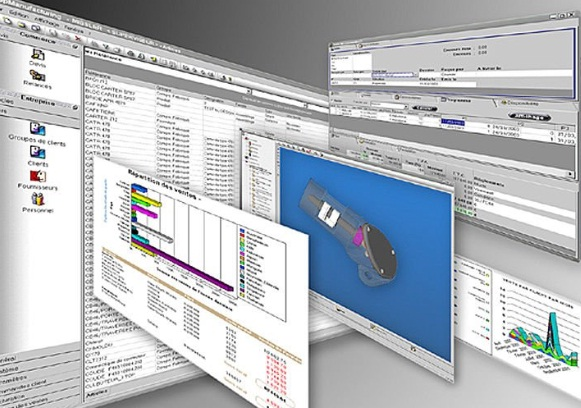
\includegraphics[width=.75\textwidth]{figures/software/software.jpg}
  \caption{Ini adalah contoh software}\label{fig:software}
\end{figure}


\subsubsection{Perngertian Software Menurut Para Ahli}

\begin{enumerate}
\item Menurut Wiwit Siswoutomo, software adalah nyawa dari sebuah hardware atau komputer karena tanpa adanya perangkat lunak maka komputer hanyalah sebuah hardware yang mati dan tidak dapat digunakan.

\item Menurut Roger S. Pressman (2002), pengertian software adalah suatu perintah program dalam sebuah komputer yang apabila dieksekusi oleh usernya akan memberikan fungsi dan unjuk kerja seperti yang diharapkan oleh user-nya. Dengan kata lain, perangkat lunak berfungsi untuk memberi perintah kepada komputer agar dapat berfungsi secara optimal sesuai dengan perintah user.

\item Menurut Melwin Syafrizal Daulay (2007), pengertian software adalah suatu perangkat yang berfungsi sebagai pengatur aktivitas kerja komputer dan seluruh intruksi yang mengarah pada sistem komputer dan menjembatani interaksi antara user dengan komputer.

\item Menurut Imam Prayogo Pujiono, pengertian perangkat lunak adalah suatu program dalam komputer yang dirancang sedemikian rupa, yang jika dijalankan akan memberikan perintah ke komputer/ hardware/ software lain dalam rangka menyelesaikan sebuah tugas, pekerjaan, dan juga tuntutan tertentu seperti yang diharapkan user.

\item Menurut Wilman dan Riyan, pengertian software adalah sebuah perangkat operasi kerja untuk menjalankan berbagai komponen pada hardware yang memiliki sifat maya (tidak terlihat) tetapi bermanfaat bagi user-nya.
\end{enumerate}

\subsubsection{Fungsi Software}

Pada dasarnya fungsi utama software adalah untuk membuat sebuah komputer dapat menjalankan perintah dari user. Mengacu pada pengertian software yang dijelaskan di atas, adapun beberapa fungsi software adalah sebagai berikut:

\begin{enumerate}
\item Menyediakan fungsi dasar dari sebuah komputer sehingga dapat dioperasikan. Misalnya ketersediaan sistem operasi dan sistem pendukung pada komputer.

\item Mengatur setiap hardware yang ada pada komputer sehingga dapat bekerja secara simultan.

\item Menjadi penghubung antara beberapa perangkat lunak lainnya dengan hardware yang ada pada komputer.

\item Perangkat lunak juga berfungsi sebagai penerjemah suatu perintah software lainnya ke dalam bahasa mesin, sehingga dapat dimengerti oleh hardware.

\item Software juga dapat mengidentifikasi suatu program yang ada pada sebuah komputer.
\end{enumerate}

\subsubsection{Software Berdasarkan Jenisnya}

\begin{itemize}

\item Operating System (sistem operasi), yaitu perangkat lunak yang berfungsi untuk mengelola dan mengkoordinasikan setiap komponen dan fungsi komputer. Beberapa contoh operating sistem adalah; Windows, Linux, UNIX, DOS.

\item Programming Language (Bahasa Pemrograman), yaitu perangkat lunak yang berfungsi sebagai pemberi instruksi standar yang melibatkan sintak dan semantik yang dipakai untuk mendefinisikan suatu program aplikasi komputer (computer application program). Beberapa contoh Bahasa Pemrograman adalah; PHP, Java, Microsoft Visual Basic.

\item Application Program (Program Aplikasi), yaitu perangkat lunak yang memiliki fungsi tertentu, misalnya software untuk presentasi, software akuntansi, dan lain sebagainya. Beberapa contoh Program Aplikasi adalah; Microsoft Office Word, Microsoft Office Excel, MYOB, OpenOffice.org, dan lainnya.
\end{itemize}

\subsubsection{Software Berdasarkan Distribusinya}

\begin{itemize}
\item Freeware, yaitu perangkat lunak yang dapat dimiliki dan digunakan secara gratis tanpa batas waktu tertentu. Biasanya perangkat lunak jenis ini memiliki fitur yang kurang lengkap dan tidak maksimal.

\item Adware, yaitu software yang bisa didapatkan dan digunakan secara gratis namun dengan kompensasi adanya iklan yang muncul di komputer user.

\item Spyware, yaitu perangkat lunak yang dibuat khusus untuk memata-matai segala aktivitas pengguna komputer. Biasanya software jenis ini banyak disalahgunakan, misalnya untuk mencuri data dari komputer lain.

\item OpenSource, yaitu software yang kode sumbernya dapat dibuka, diubah-ubah, ditingkatkan, dan disebarluaskan. Biasanya software jesni ini dapat diperoleh secara gratis dan dapat dikembangkan oleh orang lain dengan lisensi GPL (General Public License).

\item Shareware, yaitu piranti lunak untuk keperluan tertentu yang dibagikan secara gratis, biasanya sebagai demonstrasi dengan fitur terbatas dan penggunaannya untuk waktu terbatas (misalnya 30 hari).

\end{itemize}

\subsection{Hardware}

Perangkat keras komputer adalah semua bagian fisik komputer, dan dibedakan dengan data yang berada di dalamnya atau yang beroperasi di dalamnya, dan dibedakan dengan perangkat lunak (software) yang menyediakan instruksi untuk perangkat keras dalam menyelesaikan tugasnya.

Hardware dalam bahasa Indonesia disebut juga dengan nama “perangkat keras” yaitu salah satu komponen dari sebuah komputer yang sifat alatnya bisa dilihat dan diraba secara langsung atau yang berbentuk nyata, yang berfungsi untuk mendukung proses komputerisasi. Hardware dapat bekerja berdasarkan perintah yang telah ditentukan atau disebut juga dengan istilah “instruction set”. Adanya perintah yang dapat dimengerti oleh hardware, maka hardware tersebut dapat melakukan berbagai kegiatan yang telah ditentukan oleh pemberi perintah.

Secara fisik, Komputer terdiri dari beberapa komponen yang merupakan suatu sistem. Sistem adalah komponen-komponen yang saling bekerja sama membentuk suatu kesatuan. Apabila salah satu komponen tidak berfungsi, akan mengakibatkan tidak berfungsinya proses-proses yang ada pada komputer dengan baik. Komponen komputer ini termasuk dalam kategori elemen perangkat keras (hardware). Berdasarkan fungsinya, perangkat keras komputer dibagi menjadi 3 :

\begin{enumerate}

\item Input Device (unit masukan)

Unit ini berfungsi sebagai media untuk memasukkan data dari luar ke dalam suatu memori dan processor untuk diolah guna menghasilkan informasi yang diperlukan. Data yang dimasukkan ke dalam sistem komputer dapat berbentuk signal input dan maintenance input. Signal input berbentuk data yang dimasukkan ke dalam sistem komputer. Sedangkan maintenance input berbentuk program yang digunakan untuk mengolah data yang dimasukkan.

Jadi, Input device selain digunakan untuk memasukkan data dapat pula digunakan untuk memasukkan program. Berdasarkan sifatnya, peralatan input dapat digolongkan menjadi 2 yaitu :

\begin{itemize}
\item Peratalan input langsung, yaitu input yang dimasukkan langsung diproses oleh alat pemroses. Contohnya : keyboard, mouse, touch screen, light pen, digitizer graphics tablet, scanner.

\item Peralatan input tidak langsung, input yang melalui media tertentu sebelum suatu input diproses oleh alat pemroses. Contohnya : punched card, disket, harddisk.
\end{itemize}

\item Process Device (Unit Pemrosesan)

Perangkat pengolah data dipergunakan untuk mengolah data. Pengolah data meliputi unit pengolah pusat (CPU/Central Processing Unit) dan juga mikroprosesor. CPU (Central Processing Unit) merupakan alat yang berfungsi sebagai pemroses data. CPU berisi rangkaian sirkuit yang menyimpan instruksi-instruksi pemrosesan dan penyimpanan data.

Beberapa sirkuit tersebut terdapat Motherboard, Processor, Memory (RAM), Kartu Grafis (VGA Card), Kartu Suara (Sound Card), Harddisk, Floopy Disk Drive, DVD Room, Power Supply, Baterai CMOS, Fan, Heatsink, dll. 

Unit pemrosesan yang berada dalam komputer adalah Central Processing Unit (CPU). CPU merupakan otak atau pengatur suatu sistem yang mengolah sehingga menghasilkan informasi. 

Ada tiga unsur penting yang ada dalam CPU :

\begin{itemize}
\item Primary storage adalah ukuran besarnya processor atau biasa disebut dengan main memory.
\item Arithmatic logic unit adalah suatu alat yang bertugas melakukan perhitungan dalam komputer
\item Control unit adalah merupakan suatu alat pengontrolan yang berada dalam komputer yang memberitahukan unit masukan mengenai jenis data, waktu pemasukan, dan tempat penyimpanan didalam primary storage. Control unit juga bertugasmemberitahukan kepada arthmaticlogic unit mengenai operasi yang harus dilakukan, tempat data diperoleh, dan letak hasil ditempatkan.
\end{itemize}

\item Output Device (Unit Keluaran)

\begin{enumerate}

\item Printer
Printer merupakan alat pencetak dengan media kertas, hasil yang terdapat dalam komputer adalah berbentuk softcopy agar bisa di lihat tanpa menggunakan komputer maka perlu dicetak di kertas dengan printer.Komponen : Drum, Toner, Corona wire, Fuser, Laser scanner, Roller.


\end{enumerate}
\end{enumerate}



\chapter{Kernel dan Perintah Dasar}
\section{Kernel}
Perintah navigasi direktori

\section{Struktur direktori dan perintah dasar setiap sistem operasi}
Perintah navigasi direktori

\chapter{CPU}
\section{Arsitektur dan fungsi CPU}
\subsection Pengertian CPU 
CPU/Central Processing Unit adalah perangkat keras komputer yang mempunyai fungsi untuk menerima dan melakukan perintah dan data dari perangkat lunak. Karena merupakan pusat pengolahan data dalam sebuah komputer, CPU sering disebut sebagai processor. Cepat atau lambatnya kinerja dari sebuah komputer salah satunya dapat dilihat dari kualitas dan teknologi dari CPU yang digunakan.

\subsection KOMPONEN UTAMA CPU
Arihtmetic Logikal Unit (ALU). Fungsinya :
\begin{enumerate}
\item Melakukan komputasi untuk pengolahan data.
\item Melakukan tugas-tugas dasar aritmatik dan operasi logika.
\end{enumerate}

Control Unit. Fungsinya : 
\begin{enumerate}
\item  Mengatur dan mengendalikan alat-alat masukan (input) dan keluaran (output).
\item Mengambil instruksi-instruksi dari memori utama.
\item Mengambil data dari memori utama (jika diperlukan) untuk diproses.
\item Mengirim instruksi ke ALU apabila ada perhitungan aritmatika atau perbandingan logika serta mengawasi kerja dari ALU.
\item Menyimpan hasil proses ke memori utama.
\end{enumerate}

Register, fungsinya :
Memori internal yang didesain untuk dapat menyimpan data lebih cepat dibandingkan memori utama

Internal Bus, fungsinya :
Jalur yang berfungsi sebagai jembatan komunikasi antara komponen utama




\chapter{Memori}
\section{Manajemen Memori}
\par
Kinerja komputer sangat dipengaruhi oleh Organisasi dan manajemen memori.
Manajemen memori melakukan tugas yang penting dan sangat komplek berkaitan dengan :
\begin{enumerate}
\item Memori utama sebagai sumber daya yang harus dialokasikan dan dipakai bersama antar sejumlah proses yang aktif
\item Upaya agar pemrogram atau proses tidak dibatsi kapasitas memori fisik di sistem komputer.
\end{enumerate}

Fungsi Manajemen memori 
\begin{enumerate}
\item mengelola informasi memori yang dipakai dan tidak dipakai
\item mengalokasikan memori ke proses yang memerlukan
\item Mendealokasikan memori dari proses telah selesai.
\item Memgelola swapping antar memori utama dan disk
\end{enumerate}

\section{Jenis Memori}
\subsection{Jenis Memori Yang Populer}

Berikut ini beberapa jenis memori yang banyak digunakan pada saat ini sebagai berikut:

\begin{enumerate}

\item RAM (Random Acces Memory) adalah memory sebagai tempat penyimpanan sementara pada saat komputer di jalankan dan dapat di akses secara acak atau random. Fungsi dari RAM adalah mempercepat pemrosesan data pada komputer. Semakin tinggi jumlah RAM yang Anda miliki, semakin cepat pula kemampuan komputer Anda dalam mengeksekusi.
Jenis Memory RAM :

\begin{itemize}

\item EDORAM (Extended Data Out RAM)  
\item SDRAM (Synchronous Dynamic RAM)  
\item DDR SDRAM (Double Data Rate Synchronous Dynamic RAM) 
\item RDRAM (Rambus Dynamic RAM)

\end{itemize}	

\item Menurut artikel yang berjudul Evolusi Komputer, Kinerja Komputer Dan Interconnection Networks Dalam Perkembangan Dunia Teknologi Informatika menyebutkan bahwa Registers adalah media penyimpan internal CPU yang digunakan saat proses pengolahan data. Memori ini bersifat sementara, biasanya hanya digunakan untuk menyimpan data saat diolah ataupun data untuk pengolahan selanjutnya. Sistem dan bus yang menghubungkan komponen-komponen eksternal CPU dengan sistem lain, seperti memori utama serta piranti masukan atau keluaran dan juga menghubungkan komponen – komponen internal CPU dengan system lain, seperti Arimathics Logics Unit, Unit Control, dan Registers system koneksi dan bus tersebut disebut CPU Interconnections. \cite{junior2016evolusi}

\item Menurut artikel yang berjudul Evolusi Komputer, Kinerja Komputer Dan Interconnection Networks Dalam Perkembangan Dunia Teknologi Informatika menyebutkan bahwa Read Only Memory disingkat ROM merupakan memori yang tidak dapat dihapus isinya, hanya dapat dibaca, dan sudah diisi oleh pabrik pembuat komputer atau bisa dikatakan tidak bisa diprogram kembali. Sebagian perintah pada ROM akan dipindahkan ke RAM. Perintah yang ada di ROM antara lain, perintah untuk menampilkan pesan dilayar, perintah untuk membaca Sistem Operasi dari disk, dan perintah untuk mengecek semua peralatan yang ada di Unit Sistem.
Perkembangan ROM (Read Only Memory)
- Programble ROM disingkat PROM merupakan ROM yang bisa diprogram kembali dengan catatan hanya bisa diprogram 1 x.
- Re-Programble ROM disingkat RPROM merupakan ROM yang bisa diprogram ulang sesuai dengan yang kita inginkan.
- Eraseble Programble ROM disingkat EPROM merupakan ROM yang dapat dihapus dan diprogram kembali tetapi cara penghapusannya dengan menggunakan Sinar Ultraviolet.
- Electrically Eraseble Programble ROM disingkat EEPROM merupakan ROM yang bisa diprogram dengan Teknik Elektronik. \cite{junior2016evolusi}

\item Dynamic RAM disingkat DRAM merupakan salah satu jenis RAM yang harus disegarkan secara berkala oleh CPU supaya data yang terkandung di dalamnya tidak hilang. DRAM merupakan salah satu tipe RAM yang terdapat dalam PC.
Compmentary Meta-Oxyde Semiconductor disingkat CMOS merupakan jenis chip yang memerlukan daya listrik dari baterai. Chip ini berisi memori 64-byte yang isinya dapat diganti. Chip ini biasanya mengatur berbagai pengaturan - pengaturan dasar yang terdapat 
pada perangkat komputer, seperti piranti yang digunakan untuk memuat sistem operasi dan termasuk pula tanggal dan jam sistem. CMOS merupakan bagian dari ROM. Dibawah ini merupakan gambar DRAM
\ref{labelgambar1}
\begin{figure}[htbp]
\centering
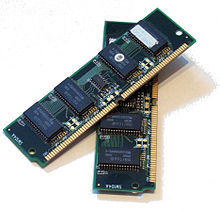
\includegraphics[width=0.45\textwidth]{figures/image/DRAM.jpg}
\caption{DRAM}
\label{labelgambar1}
\end{figure}

\item Sychronous Dynamic RAM disingkat SDRAM merupakan kelanjutan dari DRAM tetapi memiliki kecepatan yang lebih tinggi daripada DRAM dan telah disinkronisasi oleh clock sistem. DRAM ini cocok digunakan untuk sistem dengan bus yang memiliki kecepatan sampai 100 MHz. Dibawah ini merupakan gambar SDRAM
\ref{labelgambar2}
\begin{figure}[htbp]
\centering
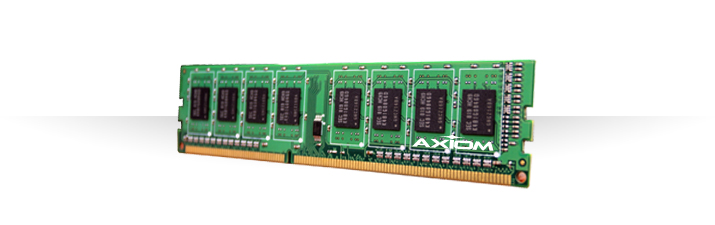
\includegraphics[width=0.45\textwidth]{figures/image/sdram.jpg}
\caption{SDRAM}
\label{labelgambar2}
\end{figure}

\item Dual In-line Memory Module disingkatan DIMM dari  berkapasitas 168 pin, kedua belah modul memori ini aktif, setiap permukaan adalah 84 pin. Berbeda dengan SIMM yang berfungsi hanya pada sebelah modul saja. Mensuport 64 bit penghantaran data. SDRAM
(Synchronous DRAM) menggunakan DIMM dan merupakan penganti dari DRAM, FPM (fast Page Memory) dan EDO. SDRAM memiliki fungsi untuk mengatur (synchronizes) memori supaya setara dengan CPU clock supaya pemindahan data yang dilakukan dapat dilakukan secara cepat. Terdapat dalam dua kecepatan yaitu 100MHz (PC100) dan 133MHz (PC133). DIMM 168 PIN. DIMM merupakan jenis RAM yang populer dan paling banyak terdapat di pasaran. Dibawah ini merupakan gambar DIMM
\ref{labelgambar3}
\begin{figure}[htbp]
\centering
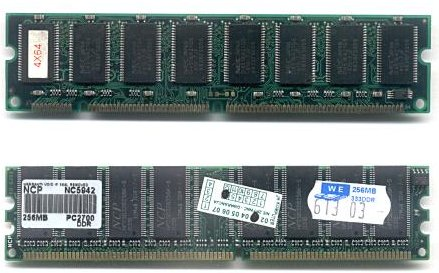
\includegraphics[width=0.45\textwidth]{figures/image/dimm.jpg}
\caption{DIMM}
\label{labelgambar3}
\end{figure}

\item Cache merupakan memori yang berkapasitas terbatas, namun memori ini memiliki kecepatan  yang tinggi dan lebih mahal dibandingkan memory utama. Cache ini terletak di antara register pemroses dan memori utama, dan memiliki fungsi agar pemroses tidak langsung mengacu kepada memori utama tetapi langsung di cache memory yang kecepatan aksesnya lebih tinggi, metode ini akan meningkatkan kinerja sistem. Cache memori merupakan salah satu tipe RAM tercepat yang pernah ada, dan digunakan oleh CPU, hard drive, dan beberapa pernah lainnya.

\item Magnetik Disk merupakan sebuah piringan bundar yang terbuat dari bahan tertentu seperti, logam atau plastik dengan permukaan dilapisi bahan - bahan yang dapat di magnetisasi. Mekanisme baca atau tulis menggunakan head atau kepala baca atau tulis yang dimana merupakan sebuah kumparan pengkonduksi (conducting coil ). Tampilan luar head bersifat stasioner sedangkan piringan disk berputar sesuai kontrolnya. Disk memiliki dua metode layout data, yaitu  constant angular velocity dan multiple zoned recording. Disk diorganisasikan dalam bentuk berupa cincin – cincin
Konsentris yang disebut track. Tiap track pada disk dipisahkan oleh gap. Gap digunakan sebagai pencegah atau mengantisipasi kesalahan penulisan maupun pembacaan yang disebabkan melesetnya head atau karena interferensi medan magnet. Sejumlah bit yang sama akan menempati track - track yang tersedia. Semakin dalam maka kerapatan dari disk akan bertambah besar. Biasanya data yang dikirim ke memori dalam bentuk blok - blok dan umumnya blok - blok tersebut lebih kecil kapasitasnya dari pada track. Blok - blok data yang disimpan dalam disk yang berukuran blok, yang disebut sektor. Sehingga track biasanya terisi beberapa sektor, umumnya 10 hingga 100 sektor tiap tracknya. Cara mekanisme pembacaan maupun penulisan pada disk dengan Head harus bisa mengidentifikasi titik awal atau posisi - posisi sektor maupun track. Caranya data yang disimpan akan diberi header data tambahan yang menginformasikan letak sektor dan track suatu data. Tipe memori Teknologi Ukuran Waktu akses Cache Memory semikonduktor RAM 128-512 KB 10 ns. Memori Utama semikonduktor RAM 4-128 MB 50 ns. Disk magnetik Hard Disk Gigabyte 10 ms, 10MB/det. Disk Optik CD-ROM Gigabyte 300ms, 600KB/det Pita magnetik Tape 100 MB De. Dibawah ini merupakan gambar Magnetik Disk
\ref{labelgambar4}
\begin{figure}[htbp]
\centering
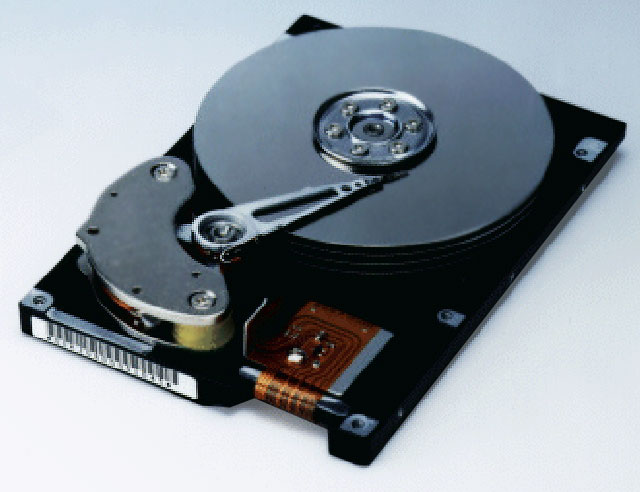
\includegraphics[width=0.45\textwidth]{figures/image/magnetic_disk.jpg}
\caption{Magnetc Disk}
\label{labelgambar4}
\end{figure}

\end{enumerate}


\section{Volatile non Volatile}
Volatile memory merupakan memory yang datanya dapat ditulis serta dihapus, tetapi akan hilang saat kehilangan power (kondisi off) serta membutuhkan suatu daya dalam mempertahankan memory. Contoh dari memory volatile yaitu RAM. RAM adalah memory utama PC yg bertugas untuk menerima sebuah informasi kemudian menyimpannya. kegunaannya sebgai penyimpanan sementara. 


Non-volatile memory merupakan memory yang datanya dapat ditulis serta dihapus, tetapi data akan tetap ada walaupun dalam kondisi off serta tidak membutuhkan suatu daya. Contoh dari memory Non volatile yaitu ROM. ROM adalah memory pada PC untuk menyimpan firmware. ROM bersifat permanen, artinya jika aliran listrik mati data yg tersimpan tidak akan terhapus


\section{Kecepatan Media Penyimpanan}
Perintah navigasi direktori

\chapter{Komunikasi Hardware}
\section{internal BUS}
Perintah navigasi direktori

\section{komunikasi Eksternal}
Perintah navigasi direktori




\chapter{Bilangan Komputasi}
\section{Biner}
\subsection{Pengertian Bilangan Biner atau Binary}
Bilangan biner atau bisa juga disebut bilangan binary merupakan sistem penulisan angka dengan hanya menggunkan dua simbol
yaitu 1 dan 2. bilangan biner merupakan dasardari semua sistem bilangan yang berbasis digital. dari sistem biner kita dapat
mengkonversikannya ke sistem bilangan Oktal atau Hexadesimal.

Bilangan biner umumnya digunakan dalam dunia komputasi. komputer menggunakan bilangan biner agar dapat saling berinteraksi
terhadap semua komponen (hardware) dan bisa juga berinteraksi terhadap sesama komputer. contoh nya pada sebuah komputer yaitu
apabila sebuah komputer terhubung dengan tegangan listrik maka bernilai 1 dan apabila komputer tidak terhubung dengan jaringan
listrik makanilai nya 0.

operasi bilangan biner  adalah operasi antara dua bilangan. dasar perkalian adalah tabel yang memuat hasil perkalian operasi
pada biner antara bilangan satu digit.

\subsection{Bilangan Biner}
\qquad Sebagai perumpamaan untuk bilangan desimal, untuk angka 157 : $157_{(10)}$ = (1 x 100) + (5 x 10) + (7 x 1) \\

Perhatikan! Bilangan desimal atau sering juga disebut dengan basis 10. Hal ini dikarenakan perpangkatan 10 yang didapat dari 100, 101, 102, dst.

\subsection{Mengenal Konsep Bilangan Biner dan Desimal}
\qquad Perbedaan paling mendasar dari metode bilangan biner dan bilangan desimal terletak pada jumlah dari basisnya. Jika desimal berbasis 10 (x10) berpangkatkan 10x, maka untuk bilangan biner berbasiskan 2 (x2) menggunakan perpangkatan 2x.
Sederhananya perhatikan contoh dibawah ini!\\
Untuk Desimal:
\begin{table}[!ht]
\begin{tabular}{ l l }
$14_{(10)}$ & = (1 x $10^1$) + (4 x $10^0$)\\
& = 10 + 4\\
& = 14\\
\end{tabular}
\end{table}
\\
Untuk Biner:
\begin{table}[!ht]
\begin{tabular}{ l l }
$1110_{(2)}$ & = (1 x $2^3$) + (1 x $2^2$) + (1 x $2^1$) + (0 x $2^0$)\\
& = 8 + 4 + 2 + 0\\
& = 14\\
\end{tabular}
\end{table}

Bentuk umum dari bilangan biner dan bilangan desimal bisa dilihat pada tabel \ref{table:binerdesimal}.

\begin{table}[!ht]
\centering
\begin{tabular}{ |c|c|c|c|c|c|c|c|c|c| }
\hline
Biner & 1 & 1 & 1 & 1 & 1 & 1 & 1 & 1 & 11111111 \\
\hline
Desimal & 128 & 64 & 32 & 16 & 8 & 4 & 2 & 1 & 255 \\
\hline
Pangkat & $2^7$ & $2^6$ & $2^5$ & $2^4$ & $2^3$ & $2^2$ & $2^1$ & $2^0$ & $X^{1-7}$ \\
\hline
\end{tabular}
\caption{Tabel bentuk umum dari bilangan biner dan bilangan desimal}
\label{table:binerdesimal}
\end{table}


\section{Hexadecimal}
Hexadecimal adalah sebuah sistem bilangan yang menggunakan sebuah simbol.Dalam hexadecimal Terdapat beberapa simbol yang bisa digunakan di sistem bilangan ini.Berbeda dengan bilangan decimal.hexadecimal menggunakan angka 0 sampai 1, di bilangan hexadecimal ini tidak menggunakan angka semua melainkan ada beberapa simbol yang menggunakan huruf.jumlah simbol yang yang berasal dari angka 1 sampai 9 berjumlah 16 simbol, ditambah dengan 6 simbol lainnya yang menggunakan huruf dari A sampai F.Hexadecimal bisa digunakan untuk menampilkan nilai alamat memori dan pemrograman komputer.Teknik penjumlahan dan pengurangan pada bilangan hexadecimal hampir sama dengan penjumlahan dan pengurangan pada bilangan biner,octal dan decimal, tetapi jika terjadi carry 1 atau borrow 1, maka angka 1 tersebut bernilai 16. Carry akan terjadi apabila penjumlahan lebih dari 15 misalnya 8+8=10. Sedangkan borrow terjadi apabila angka yang dikurangi lebih kecil dari pengurang, misalnya 45-6=. 

\chapter{Standar}
\section{ASCII}
Perintah navigasi direktori

\section{UTF-8}
Perintah navigasi direktori


\chapter{Serial Comm}
\section{Cara Kerja Driver}
Perintah navigasi direktori

\section{Serial Monitor}
Perintah navigasi direktori


\chapter{Arduino}
\section{Struktur Arduino}
\subsection{Pengertian Arduino UNO}
Arduino adalah pengendali mikro single-board yang bersifat open-source, diturunkan dari Wiring platform, dirancang untuk memudahkan penggunaan elektronik dalam berbagai bidang. Arduino UNO merupakan sebuah board mikrokontroler yang dikontrol penuh oleh ATmega328.

\subsection{Kegunaan Arduino UNO}
Arduino dapat disambungkan dan mengontrol led, beberapa led, bahkan banyak led, motor DC, relay, servo, modul dan sensor-sensor, serta banyak lagi komponen lainnya.

\section{Digital Analog}
Perintah navigasi direktori

\section{IDE}
Perintah navigasi direktori

\section{Membuat Rancangan Rangkaian}
    Membuat rangkaian dapat dilakukan dengan bantuan aplikasi simulator contohnya VBB (Virtual Bread Board).
\begin{figure}[!htbp]
  \centering
  
\includegraphics[width=.45\textwidth]{figures/VBB/vbb.png}
  \caption{Ini adalah aplikasi VBB}\label{fig:vbb}
\end{figure}

Bagaimana cara install VBB?
\begin{enumerate}
\item Download installer vbb

\item Double-click installer vbb,seperti pada gambar \ref{fig:installer}
\begin{figure}[!htbp]
  \centering
  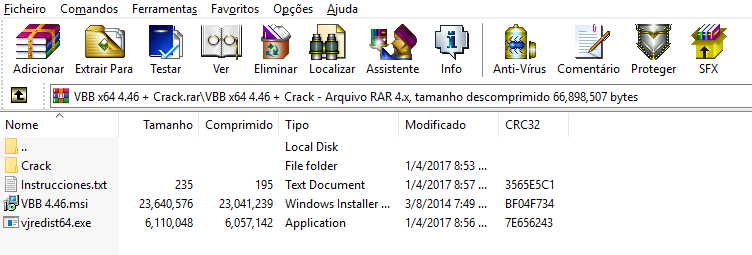
\includegraphics[width=.75\textwidth]{figures/VBB/installer.png}
  \caption{Ini adalah installer}\label{fig:installer}
\end{figure}

\item Maka akan tampil seperti gambar \ref{fig:halawalinstallasi}
\begin{figure}[!htbp]
  \centering
  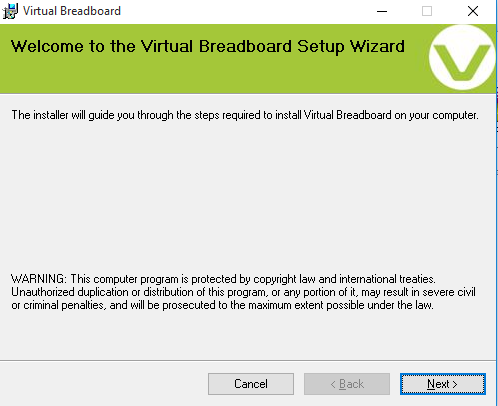
\includegraphics[width=.75\textwidth]{figures/VBB/halawalinstallasi.png}
  \caption{Ini adalah Halaman Awal Installasi}\label{fig:halawalinstallasi}
\end{figure}

\item Pilih direktori penyimpanan seperti gambar \ref{fig:memilihdirektori}
\begin{figure}[!htbp]
  \centering
  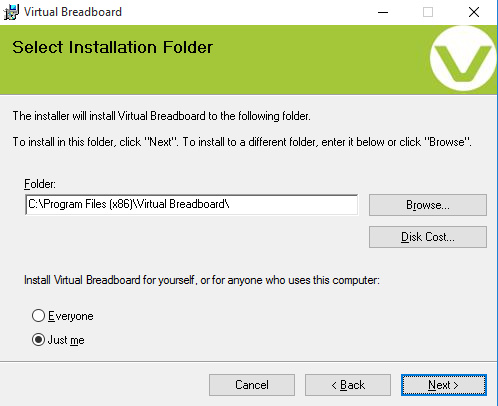
\includegraphics[width=.75\textwidth]{figures/VBB/memilihdirektori.png}
  \caption{Ini adalah Halaman Pemilihan Direktori}\label{fig:memilihdirektori}
\end{figure}


\item Kemudian tekan tombol next, maka akan muncul halaman konfirmasi seperti pada gambar \ref{fig:konfirmasiinstall}
\begin{figure}[!htbp]
  \centering
  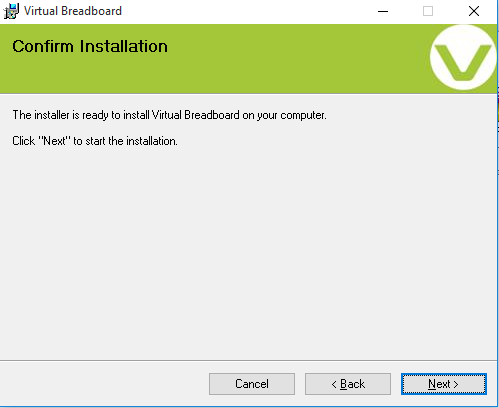
\includegraphics[width=.75\textwidth]{figures/VBB/konfirmasiinstall.png}
  \caption{Ini adalah Halaman Konfirmasi Installasi}\label{fig:konfirmasiinstall}
\end{figure}

\item Lalu tunggu sampai proses installasi selesai, seperti pada gambar \ref{fig:prosesinstallasi}
\begin{figure}[!htbp]
  \centering
  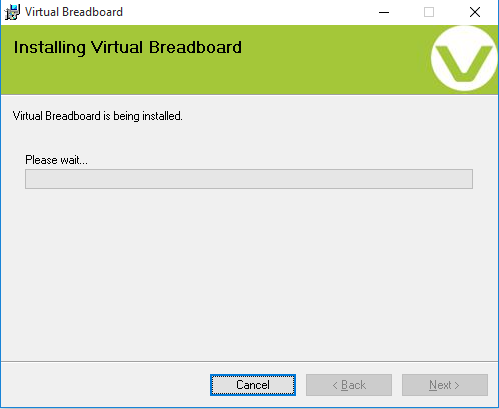
\includegraphics[width=.75\textwidth]{figures/VBB/prosesinstallasi.png}
  \caption{Ini adalah Proses Installasi}\label{fig:prosesinstallasi}
\end{figure}

\item Proses installasi selesai, seperti pada gambar \ref{fig:installasiselesai}
\begin{figure}[!htbp]
  \centering
  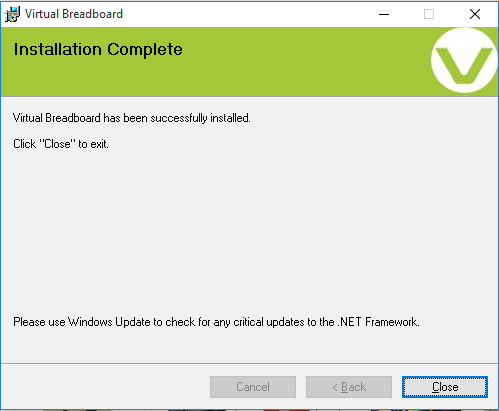
\includegraphics[width=.75\textwidth]{figures/VBB/installasiselesai.png}
  \caption{Ini adalah Proses Installasi Telah Selesai}\label{fig:installasiselesai}
\end{figure}
\end{enumerate} 

\chapter{Perintah Sederhana}
\section{Menyalakan LED menggunakan Arduino}
Perintah navigasi direktori

\section{1-3 LED bergantian}
Perintah navigasi direktori


\chapter{Feedback Sensor}
\section{Berbagai macam Jenis Sensor}
\section{Pengertian Sensor Suara}
Sensor suara merupakan sensor yang mensensing besaran suara untuk diubah menjadi besaran listrik. Sensor ini bekerja berdasarkan besar kecilnya kekuatan gelombang suara yang diterima. Dimana gelombang suara tersebut mengenai membran sensor, yang menyebabkan bergeraknya membran sensor yang memiliki kumparan kecil sehingga menghasilkan besaran listrik. Kecepatan bergeraknya kumparan kecil tersebut menentukan kuat lemahnya gelombang listrik yang akan dihasilkan. Salah satu contoh komponen yang termasuk dalam sensor ini adalah condeser microphone atau mic. Bentuk fisik dari condeser mic yaitu berbentuk bulat dan memiliki kaki dua seperti contoh pada gambar \ref{fig:sscondesermic}.
\begin{figure}[!htbp]
  \centering
  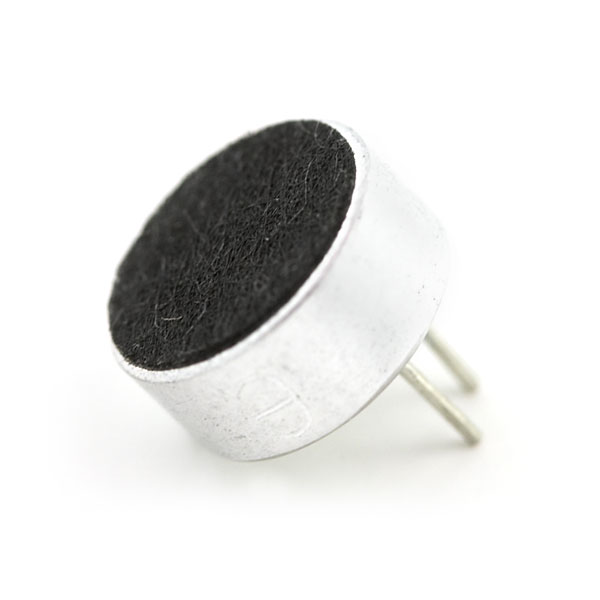
\includegraphics[width=.75\textwidth]{figures/Arduino/sscondesermic.jpg}
  \caption{Ini adalah Condeser Microphone}\label{fig:sscondesermic}
\end{figure}

\subsection{Prinsip Kerja Condeser Microphone}
Condenser mic biasanya bekerja berdasarkan susunan backplate atau diafragma yang harus terhubung dengan listrik dan membentuk kapasitor sound - sensitive. Gelombang suara yang tercipta akan masuk ke microphone dan akan menggetarkan komponen diafragma ini. Letak dari diafragma ditempatkan di depan sebuah backplate. Susunan dari elemen - elemen tersebut akan membentuk sebuah kapasitor yang sering disebut juga sebagai kondenser. Kapasitor memiliki kemampuan untuk menyimpan muatan maupun tegangan. Ketika elemen tersebut terisi dengan muatan, medan listrik akan terbentuk di antara diafragma dan backplate, yang dimana besarnya itu proporsional terhadap ruang yang terbentuk diantaranya. Macam - macam lebar dari jarak antara backplate dengan diafragma yang terjadi disebabkan karena adanya pergerakan oleh diafragma relatif terhadap backplate yang dikarenakan adanya tekanan suara yang mengenai diafragma. Hal ini akan menghasilkan sinyal elektrik dari gelombang suara yang masuk ke condenser microphone seperti contoh pada gambar \ref{fig:sscondesermicscheme}.
\begin{figure}[!htbp]
  \centering
  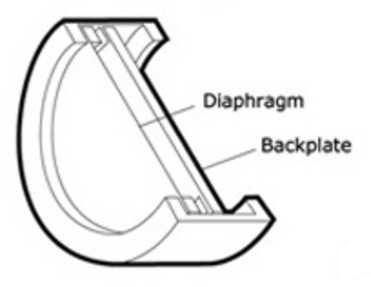
\includegraphics[width=.75\textwidth]{figures/Arduino/sscondesermicscheme.jpg}
  \caption{Ini adalah Skema dari Condeser Microphone}\label{fig:sscondesermicscheme}
\end{figure}

\subsection{Karakteristik dari Condeser Microphone}

Karakteristik dari Conseder Microphone adalah sebagai berikut :

\begin{enumerate}
  \item Susunannya lebih kompleks dibanding dengan jenis microphone lainnya seperti dibanding dengan dynamic Microphone.
  \item Pada frekuensi tinggi, akan menghasilkan suara yang lebih halus dan natural, serta sensitivitas yang lebih tinggi.
  \item Mudah akan mencapai respon frekuensi flat dan memiliki range frekuensi yang lebih luas.
  \item Ukurannya lebih kecil dibanding dengan jenis tipe mikrophone lainnya.
\end{enumerate}

Pada pasaran sudah dijual sensor suara menggunakan condeser mic ini dalam bentuk modul, sehingga mudah dan praktis dalam penggunaannya.

\begin{figure}[!htbp]
  \centering
  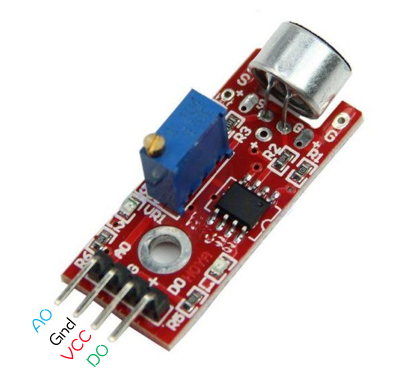
\includegraphics[width=.75\textwidth]{figures/Arduino/sssensorsuara.png}
  \caption{Ini adalah Skema dari Condeser Microphone}\label{fig:sssensorsuara}
\end{figure}	

Spesifikasi dari modul sensor suara seperti contoh pada gambar \ref{fig:sssensorsuara} adalah sebagai berikut :

\begin{enumerate}
  \item Sensitivitas dapat diatur (pengaturan manual pada potensiometer).
  \item Condeser yang digunakan memiliki sensitivitas yang tinggi.
  \item Tegangan kerja antara 3.3V – 5V.
  \item Terdapat 2 pin keluaran yaitu tegangan analog dan digital output.
  \item Sudah terdapat lubang baut untuk instalasi.
  \item Sudah terdapat indikator led.
\end{enumerate} 

\section{Sensor Gas}
\begin{figure}[!htbp]
  \centering
  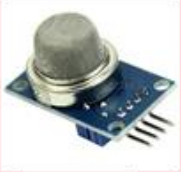
\includegraphics[width=.75\textwidth]{figures/mq2.png}
  \caption{Ini adalah Sensor suhu MQ-2 \cite{himawan2017perancangan}}\label{fig:mq2}
\end{figure}	
Sensor yang digunakan kali ini adalah sensor MQ-2 seperti pada gambar \ref{fig:mq2}, sensor ini digunakan untuk mendeteksi gas LPG, i-butana, propana, alkohol, hidroge, dan asap. Inti dari MQ-2 adalah material yang sensitif terhadap konsentrasi gas yang tersusun dari senyawa SnO2 atau Timah Oksida. Material ini mempunyai karakteristik yang akan merubah konduktivitasnya seiring dengan perubahan konsenterasi gas.
Seri MQ sensor gas menggunakan pemanas kecil di dalamnya dengan sensor elektro-kimia. Mereka sensitif terhadap berbagai gas dan digunakan di dalam ruangan pada suhu kamar.
Mereka dapat dikalibrasi lebih atau kurang lihat bagian tentang Load-resistor dan Burn-in namun diketahui konsentrasi gas atau gas yang diukur diperlukan untuk itu.
Outputnya adalah sinyal analog dan bisa dibaca dengan input analog Arduino.
Sedangkan untuk spesifikasi sensor MQ-2, adalah:
\begin{itemize}
\item suhu 20 derajat Celcius
\item kelembaban udara 65 persen
\end{itemize}
range konsentrasi gas yang bisa diukur:
\begin{itemize}
\item LPG dan propana: 200ppm-5000ppm
\item butana: 300ppm-5000ppm
\item metana: 5000ppm - 20000ppm
\end{itemize}

\section{Sensor Infrared}
\subsection{Infrared Obstacle Detector}
\begin{figure}[!htbp]
  \centering
  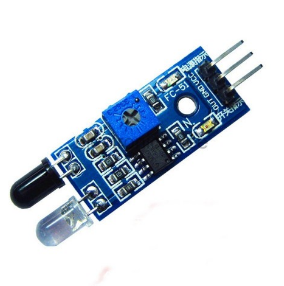
\includegraphics[width=.75\textwidth]{figures/Arduino/sensorinfrared.png}
  \caption{Ini adalah Sensor Infrared Obstacle Detector}\label{fig:obstacle}
\end{figure}
Sensor infrared obstacle detector seperti pada gambar \ref{fig:obstacle} memanfaatkan kondisi apabila infrared pada sensor ditutup maka LED notifikasi akan menyala, sensor ini bekerja dengan memanfaatkan infrared, apabila cahaya infrared diterima dengan cahaya yang cukup terang maka lampu tidak menyala dan apabila cahaya infrared diterima dengan pencerahan cahaya yang kurang maka lampu akan menyala sebagai pengganti penerangan. Kegunaan dari Infrared Obstacle Detector digunakan untuk mendeteksi penerangan cahaya dengan memanfaatkan sinar infrared yang ada pada sensor tersebut. Cara kerja dari Infrared Obstacle Detector yaitu apabila ada penghalang yang menghalangi sinar infrared maka LED notifikasi akan menyala.

\section{Sensor Cahaya}
\begin{figure}[!htbp]
  \centering
  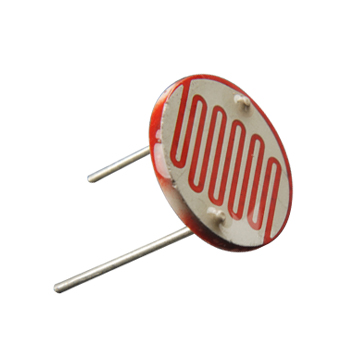
\includegraphics[width=.75\textwidth]{figures/Arduino/LDR.jpg}
  \caption{Ini adalah Sensor LDR}\label{fig:ldr}
\end{figure}

\subsection{Pengertian}
Sensor cahaya atau LDR merupakan sensor yang di pakai untuk mengubah besaran listrik menjadi besaran cahaya atau pengertian lain adalah  sensor yang membuat kita dapat melakukan pendeteksian cahaya, dan melakukan perubahan terhadap cahaya tersebut ,jadi sinyal listrik dan dipakai dalam sebuah rangkaian yang menggunakan cahaya sebagai alat pemicunya. Prinsip-prinsip kerja dari alat tersebut adalah untuk mengubah suatu energi dari foton menjadi elektron. Idealnya satu foton dapat membangkitkan satu elektron. Sensor cahaya sangat banyak penggunaannya, salah satu yang paling populer adalah kamera digital. Pada saat ini sudah ada alat yang digunakan untuk mengukur cahaya yang mempunyai 1 buah foton saja.

\subsection{Karakteristik Sensor}
Sensor Cahaya LDR (Light Dependent Resistor) merupakan suatu bentuk komponen yang mempunyai perubahan resistansi yang besarnya tergantung pada cahaya. Karakteristik LDR terdiri dari dua macam yaitu yang pertama Laju Recovery dan Respon Spektral.

Karakteristik sensor LDR adalah sebagai berikut :

\begin{itemize}
	\item LDR tipe arus harganya lebih besar dari 200K/detik.
	\item tidak mempunyai sensitivitas yang sama untuk setiap panjang gelombang cahaya yang jatuh padanya (yaitu warna).
	\item Dalam keadaan gelap resistansi LDR seki-tar 10MΩ dan dalam keadaan terang sebe-sar 1KΩ atau kurang.
\end{itemize}




\chapter{Membangun Alat}
\section{Arduino dengan LED dan Sensor}
Perintah navigasi direktori


\chapter{Aktuator}
\section{Motor DC}
Perintah navigasi direktori


\chapter{Instructables}
\section{Definisi dan Sejarah}
Perintah navigasi direktori


\bibliographystyle{IEEEtran}
%\def\bibfont{\normalsize}
\bibliography{references}


%%%%%%%%%%%%%%%
%%  The default LaTeX Index
%%  Don't need to add any commands before \begin{document}
\printindex

%%%% Making an index
%%
%% 1. Make index entries, don't leave any spaces so that they
%% will be sorted correctly.
%%
%% \index{term}
%% \index{term!subterm}
%% \index{term!subterm!subsubterm}
%%
%% 2. Run LaTeX several times to produce <filename>.idx
%%
%% 3. On command line, type  makeindx <filename> which
%% will produce <filename>.ind
%%
%% 4. Type \printindex to make the index appear in your book.
%%
%% 5. If you would like to edit <filename>.ind
%% you may do so. See docs.pdf for more information.
%%
%%%%%%%%%%%%%%%%%%%%%%%%%%%%%%

%%%%%%%%%%%%%% Making Multiple Indices %%%%%%%%%%%%%%%%
%% 1.
%% \usepackage{multind}
%% \makeindex{book}
%% \makeindex{authors}
%% \begin{document}
%%
%% 2.
%% % add index terms to your book, ie,
%% \index{book}{A term to go to the topic index}
%% \index{authors}{Put this author in the author index}
%%
%% \index{book}{Cows}
%% \index{book}{Cows!Jersey}
%% \index{book}{Cows!Jersey!Brown}
%%
%% \index{author}{Douglas Adams}
%% \index{author}{Boethius}
%% \index{author}{Mark Twain}
%%
%% 3. On command line type
%% makeindex topic
%% makeindex authors
%%
%% 4.
%% this is a Wiley command to make the indices print:
%% \multiprintindex{book}{Topic index}
%% \multiprintindex{authors}{Author index}

\end{document}

